\documentclass[twocolumn,10pt]{article}

\usepackage[utf8]{inputenc}
\usepackage{amsmath, amssymb, amsfonts, amsthm}
\usepackage{upgreek}
\usepackage{amsthm}
\usepackage{fullpage}
\usepackage{graphicx}
\usepackage{cancel}
\usepackage{subfigure}
\usepackage{mathrsfs}
\usepackage{enumerate}
%\usepackage{outlines}
\usepackage[font={sf,it}, labelfont={sf,bf}, labelsep=space, belowskip=5pt]{caption}
\usepackage{hyperref}
% \usepackage{minted}

\usepackage{float}
% \floatplacement{figure}{H}

\usepackage{fancyhdr}
\usepackage[title]{appendix}
\usepackage{siunitx}

\DeclareMathOperator{\tr}{tr}
\DeclareMathOperator{\sgn}{sgn}
\DeclareMathOperator{\sinc}{sinc}
\DeclareMathOperator{\rref}{rref}
\DeclareMathOperator{\cof}{cof}

\providecommand{\abs}[1]{\lvert#1\rvert}
\providecommand{\norm}[1]{\lVert#1\rVert}
\providecommand{\dx}{\, \mathrm{d}x}
\providecommand{\dA}{\, \mathrm{d}A}
% \providecommand{\vint}[2]{\int_{#1} \! #2 \, \mathrm{d}x}
% \providecommand{\sint}[2]{\int_{\partial #1} \! #2 \, \mathrm{d}A}
\renewcommand{\div}{\nabla \cdot}
\providecommand{\e}{\epsilon}
\providecommand{\shape}{\Omega(p)}
\providecommand{\boundary}{\partial \shape}
\providecommand{\vint}[1]{\int_{\shape} \! #1 \, \mathrm{d}x}
\providecommand{\sint}[1]{\int_{\boundary} \! #1 \, \mathrm{d}A}
\providecommand{\pder}[2]{\frac{\partial #1}{\partial #2}}
\providecommand{\tder}[2]{\frac{\mathrm{d} #1}{\mathrm{d} #2}}
\providecommand{\evalat}[2]{\left.#1\right|_{#2}}
\newcommand{\defeq}{\vcentcolon=}
\newtheorem{lemma}{Lemma}
\newcommand\numberthis{\addtocounter{equation}{1}\tag{\theequation}}

\makeatletter
\usepackage{mathtools}
\newcases{mycases}{\quad}{%
  \hfil$\m@th\displaystyle{##}$}{$\m@th\displaystyle{##}$\hfil}{\lbrace}{.}
\makeatother
\DeclarePairedDelimiter\ceil{\lceil}{\rceil}
\DeclarePairedDelimiter\floor{\lfloor}{\rfloor}

\newenvironment{amatrix}[1]{%
  \left[\begin{array}{@{}*{#1}{c}|c@{}}
}{%
  \end{array}\right]
}

%% + Abtin
\usepackage{fullpage}
\usepackage[usenames,dvipsnames]{color}
\usepackage{paralist}
\usepackage{prettyref}
\newrefformat{sec}{Section~\ref{#1}}
\newrefformat{tbl}{Table~\ref{#1}}
\newrefformat{fig}{Fig.~\ref{#1}}
\newrefformat{chp}{Chapter~\ref{#1}}
\newrefformat{eqn}{Eq.~\eqref{#1}}
\newrefformat{set}{Eq.~Set~\eqref{#1}}
\newrefformat{alg}{Algorithm~\ref{#1}}
\newrefformat{apx}{Appendix~\ref{#1}}
\newcommand\pr[1]{\prettyref{#1}}

\newcommand\todo[1]{\textcolor{magenta}{\bf [TODO: #1]}}
\renewcommand\vec[1]{\ensuremath{\mathbf #1}}
\def\x{\vec{x}}
\def\y{\vec{y}}
\def\u{\vec{u}}
\def\ue{\vec{u}^\e}
\def\strain{\varepsilon}


\begin{document}
\section{Periodic Homogenization}
Considering a heterogeneous object $\Omega^\e$ with periodic
heterogeneities of size $\e$, as shown schematically in
\pr{fig:periodic}, our goal is to find the homogenized elasticity
tensor $C^H_{ijkl}$ as the effective elasticity tensor of the
microstructure. Parameter $\e$ determines the size of cell $Y$
relative to the domain $\Omega^\e$ and permits us to perform
asymptotic analysis as $\e$ goes to zero (\pr{apx:twoscale}).
\begin{figure}[!hbt]
    \centering
    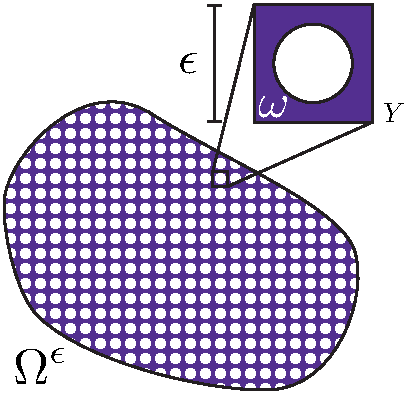
\includegraphics[width=.28\textwidth]{Images/periodic.pdf}
    \caption{(Schematic) Periodic tiling of a domain $\Omega$ with
      base cell $Y$ having geometry $\omega$ and length scale $\e$.}
    \label{fig:periodic}
\end{figure}

Let \x\ denote the macroscopic variable and define $\y\coloneqq \x/\e$
as the microscopic variable. For ${\y} \in Y$, the local elasticity
tensor is given as
\begin{equation}
  \label{eqn:microC}
  C_{ijkl} (\y) = \begin{cases} C_{ijkl}^\text{base} & \text{if } \y
  \in \omega, \\ 0 & \text{ otherwise,} \end{cases}
\end{equation}
where $C^\text{base}$ is the known material property. We extend this
function throughout $\Omega$ by Y-periodicity. The effective
elasticity tensor is derived using two-scale asymptotic analysis on
the material's elastic response and is expressed as an integral over
the cell $Y$
\begin{equation}
  \label{eqn:effective}
  C^H_{ijkl} = \frac{1}{|Y|} \int_\omega C_{ijpq}^\text{base} [\strain(\vec{w}^{kl})]_{pq} + C_{ijkl}^\text{base} \, \mathrm{d} \y,
\end{equation}
where $\strain(\vec{w})=\frac{1}{2}(\nabla \vec{w} + (\nabla
\vec{w})^T)$ is the Cauchy strain tensor and $\vec{w}^{kl}$ are the
microscopic displacements satisfying
\begin{subequations}
  \label{set:cell}
  \begin{gather}
    \nabla \cdot (C^\text{base}_{ijmn}[\strain({\bf w}^{kl})]_{mn}) = 0 \quad \text{in } \omega, \\
    C^\text{base}_{ijmn}[\strain({\bf w}^{kl})]_{mn}\hat{n}_j  =  - C^\text{base}_{ijmn}[\vec{e}^{kl}]_{mn} \hat{n}_j  \quad \text{on } \partial \omega \setminus \partial Y, \\
    {\bf w}^{kl}({\y})\ Y\text{-periodic}, \\
    \int_\omega \! {\bf w}^{kl}({\y})  \, \mathrm{d} {\y} =  {\bf 0},
  \end{gather}
\end{subequations}
where $\vec{e}^{kl} \coloneqq \frac{1}{2} \left(\vec{e}_k \otimes
\vec{e}_l + \vec{e}_l \otimes \vec{e}_k \right)$ are the canonical
basis for symmetric rank 2 tensors. See \pr{apx:twoscale} for more
detail on the derivation of \pr{eqn:effective} and \pr{set:cell}.

For each cell shape, \pr{set:cell} needs to be solved numerically for
the six\footnote{instead of nine because of the symmetry in canonical
  basis $\vec{e}^{kl} = \vec{e}^{lk}$.} cell problems to compute
$\vec{w}^{kl}\;(k,l=1,2,3)$, which are in turn used to evaluate
\pr{eqn:effective}.

\subsection{FEM Implementation}
The cell problems (\pr{set:cell}) are solved numerically by FEM
discretization of a single base cell. The volume integral
(\pr{eqn:effective}) is computed on the same grid.

Two FEM implementations are used:
\begin{inparaenum}[(i)]
\item a traditional volume mesh discretization using linear
  tetrahedron elements, and
\item a novel ``mesh free'' method using a grid of trilinear cubes not
  conforming to the object's boundary.
\end{inparaenum}
The mesh free method works directly on an object's level set
description and is more suited for tasks such as shape or topology
optimization where the object will change frequently and remeshing is
intractable.

The linear elasticity solver needs to support periodic boundary
conditions, which requires the tet-based volume mesh to have identical
tessellation on opposite periodic cell faces. The mesh free method has
matching grid on periodic faces by construction and only requires the
geometry itself to be periodic. Periodic boundary conditions are
implemented by direct elimination of variables. Direct elimination is
performed by assigning all mesh or grid nodes in each connected
component of the identified vertex graph the same degrees of
freedom. For example, the cell's corner nodes---if they exist---appear
as the graph's only component of size 8 and all get the same $x$, $y$,
and $z$ displacement degrees of freedom. Edge nodes will appear in a
component of size 4.

In both solvers, to simplify operations such as rank 4 tensor
inversion and double contractions, we use a symmetric tensor
flattening approach to turn rank 4 tensors into matrices and rank 2
tensors into vectors. We end up storing the elasticity tensor as a
symmetric $6\times 6$ matrix with 21 coefficients.

\appendix
\section{Two-scale Analysis\label{apx:twoscale}}
The elastic response of the material under external load $\vec{f}$
with Neumann and Dirichlet boundary condition on respectively
$\Gamma_N$ and $\Gamma_D$ is governed by linear elasticity equation
\begin{align*}
    -\nabla \cdot [C : e(\vec{u})] = \vec{f} \quad &\text{in } \Omega \\
    {\bf \hat{n}} \cdot [C : e({\bf u})] = {\bf \tau} \quad &\text{on } \Gamma_N \numberthis \label{eqn:elastostatic} \\
    {\bf u} = {\bf u}_D \quad &\text{on } \Gamma_D,
\end{align*}
where $\vec{u}$ is the displacement vector and
$e(\vec{u})=\frac{1}{2}(\nabla \vec{u} + (\nabla \vec{u})^T)$ is the
strain tensor.


One homogenization approach is based on the method of two-scale
asymptotic expansions \cite{allaire2002shape}, which is a heuristic
derivation of the homogenized elasticity tensor, but once this tensor
is found it can be rigorously justified. Further detail can be found
in \cite{allaire2002shape}, here we outline major steps in derivation
of $C^H$.

Assuming that the solution can be written as an asymptotic expansion
\[
\vec{u}^\e({\x}) = \sum_{p = 0}^{\infty} \e^p \vec{u}_p\left(\x, \y\right),
\]
with ${\bf u}_p({\x}, {\y})$ constrained to be $Y$-periodic in
${\y}$.  Each of these functions separates its dependence on $\x$
(i.e. the smoothly varying, macroscopic part) from its dependence on
$\y = \x/\e$ (the microscopic fluctuations). Plugging the series into
\pr{eqn:elastostatic} and collecting coefficients of $\e^p$ terms we
have
\begin{align}
    \e^{ 0}:\quad  &-\nabla_{\y} \cdot [C({\y}) : e_{\y}({\bf u}_2)] -
                     \nabla_{\x} \cdot [C({\y}) : e_{\y}({\bf u}_1)] -
                     \nabla_{\y} \cdot [C({\y}) : e_{\x}({\bf u}_1)] -
                     \nabla_{\x} \cdot [C({\y}) : e_{\x}({\bf u}_0)] = {\bf f}, \label{eqn:e0}\\
    \e^{-1}:\quad  &-\nabla_{\y} \cdot [C({\y}) : e_{\y}({\bf u}_1)] -
                     \nabla_{\x} \cdot [C({\y}) : e_{\y}({\bf u}_0)] -
                     \nabla_{\y} \cdot [C({\y}) : e_{\x}({\bf u}_0)] = {\bf 0}, \label{eqn:em1} \\
    \e^{-2}:\quad  &-\nabla_{\y} \cdot [C({\y}) : e_{\y}({\bf u}_0)] = {\bf 0}, \label{eqn:em2}
\end{align}
where $e_\x({\bf u}) \coloneqq \frac{1}{2} \left( \nabla_{\x} {\bf u}
+ (\nabla_{\x} {\bf u})^T \right)$ is the macroscopic strain operator
and $e_\y$ is the microscopic strain operator, defined similarly.

\pr{eqn:em2} implies that ${\bf u}_0({\x}, {\y}) = {\bf u}({\bf
  x})$, which by the Fredholm alternative is unique \cite[Lemma
  2.3.21]{allaire2002shape}.\footnote{Intuitively, \pr{eqn:em2} is a
  force balance for ${\bf u}_0$ in each instance of the periodic
  cell.} Plugging in ${\bf u}({\x})$ for ${\bf u}_0$ simplifies
(\ref{eqn:em1}) to
\begin{equation}
    \label{eqn:u1u}
    -\nabla_{\y} \cdot (C({\y}) : [e_{\y}({\bf u}_1) + e_{\x}({\bf u})]) =  {\bf 0},
\end{equation}
which uniquely defines ${\bf u}_1({\x}, {\y})$ at each point
${\x}$ up to a constant once ${\bf u}$ is known. We can express this
relationship with a rank 4 tensor $F$ such that $e_\y(\vec{u}_1) =
F:e_x(\vec(u))$ mapping macroscopic strain to microscopic fluctuation
strain. \pr{eqn:e0} uniquely defines $\vec{u}_2$ based on $\vec{u}$
and $\vec{u}_1$ if and only if the compatibility condition of the
Fredholm alternative (zero average right hand side) is
satisfied. Integrating \pr{eqn:e0}, using Divergence theorem and
periodicity of $\vec{u}_1$ and $\vec{u}_2$, we have the homogenized
force balance equation
\begin{align}
  &C^H \coloneqq \frac{1}{|Y|} \int_Y C({\y}) : F + C({\y}) \, \mathrm{d} {\y}  \\
  &C^H_{ijkl} = \frac{1}{|Y|} \int_Y C_{ijpq}({\y}) F_{pqkl} + C_{ijkl}({\y}) \, \mathrm{d} {\y}\\
  &-\nabla_{\x} \cdot \left[ C^H : e_{\x}({\bf u}) \right] = {\bf f} \quad \text{in } \Omega.
\end{align}

\subsection{Cell Problems}
All that remains is to use (\ref{eqn:u1u}) to determine rank 4 tensor $F$
appearing in $C^H$. First we introduce the canonical basis for symmetric rank 2 tensors:
$$
e^{ij} = \frac{1}{2} \left({\bf e}_i \otimes {\bf e}_j + {\bf e}_j \otimes {\bf e}_i \right)
$$
where ${\bf e}_i$ is the $i^\text{th}$ canonical basis element.Then we
can trivially expand the macroscopic strain at any point in this
basis:
$$
e_{\x}({\bf u}) = e^{ij} [e_{\x}({\bf u})]_{ij}
$$

We now take advantage of linearity to state that if Y-periodic ${\bf
w}^{ij}({\y})$ solves (\ref{eqn:u1u}) for $e_{\x}({\bf u}) = e^{ij}$:
\begin{equation}
-\nabla_{\y} \cdot (C({\y}) : [e_{\y}({\bf w}^{ij}) + e^{ij}]) = {\bf 0},
\end{equation}
Since this solution is unique up to a constant wrt. ${\y}$, we know that
$$
e_{\y}({\bf u}_1) = e_{\y}({\bf w}^{ij} [e_{\x}({\bf u})]_{ij}) = e_{\y}({\bf w}^{ij})[e_{\x}({\bf u})]_{ij},
$$
which gives us the linear map from $e_{\x}({\bf u})$ to $e_{\y}({\bf u}_1)$
\[
F_{pqkl} = [e_{\y}({\bf w}^{kl})]_{pq}
\]
Plugging this into the equation for the homogenized elasticity coefficients, we get in index notation:
\begin{equation}
    \label{eqn:Eh}
C^H_{ijkl}= \frac{1}{|Y|} \int_Y C_{ijpq}({\y}) [e_{\y}({\bf w}^{kl})]_{pq} + C_{ijkl}({\y}) \, \mathrm{d} {\y}.
\end{equation}
Thus, once we know each ${\bf w}^{ij}$, we can compute the homogenized elasticity tensor
with a simple integration over the base cell. We find these by solving the 6 cell problems:
\begin{align*}
    -\nabla_{\y} \cdot (C({\y}) : [e_{\y}({\bf w}^{ij}) + e^{ij}]) = {\bf 0} & \quad \text{in } Y \\
    {\bf w}^{ij}({\y})\ Y \text{-periodic} &     \numberthis \label{eqn:cell} \\
    \int_\omega \! {\bf w}^{ij}({\y})  \, \mathrm{d} {\y} =  {\bf 0},
\end{align*}
one for each canonical basis tensor $e^{ij}$. The last constraint is to pin
down the remaining translational degree of freedom; since we only care about
strain $e_{\y}({\bf w}^{ij})$, we can arbitrarily choose to enforce ${\bf
0}$ average displacement over the microstructure geometry.

\section{Solving the Cell Problems}
The homogenization task has now been reduced to solving 6 cell
problems. Using \pr{eqn:microC}, the traction free boundary condition
on the interior boundaries $\partial\omega \setminus \partial Y$, and
the fact that macroscopic stress $C^\text{base} : e^{ij}$ is constant
throughout the base cell, we have
\begin{subequations}
  \label{set:cell2}
  \begin{align}
    -\nabla \cdot (C^\text{base} : e({\bf w}^{ij})]) = {\bf 0} & \quad \text{in } \omega \\
      {\bf \hat n} \cdot \left[ C^\text{base} : e({\bf w}^{ij}) \right]  =  -{\bf \hat{n}} \cdot \left[ C^\text{base} : e^{ij} \right]& \quad \text{on } \partial \omega \setminus \partial Y \\
      {\bf w}^{ij}({\y})\ Y \text{-periodic} & \\
      \int_\omega \! {\bf w}^{ij}({\y})  \, \mathrm{d} {\y} =  {\bf 0},
  \end{align}
\end{subequations}


\bibliographystyle{plain}
\bibliography{References}

\end{document}
